\documentclass[11pt]{article}
\usepackage{hyperref}
\usepackage{graphicx}
\usepackage{caption}
\usepackage{geometry}
\usepackage{placeins}
\usepackage{enumitem}
\usepackage{multirow}
\usepackage{float}
\usepackage{wrapfig}
\usepackage{url}
\usepackage{amsmath}
\usepackage{algorithm}
\usepackage[backend=biber]{biblatex}
\usepackage{algpseudocode}
\usepackage{tikz}
\usepackage{schemata}
\usepackage{tabularx}
\usepackage{makecell}
\usepackage{pgfplots}
\usepackage[toc,page]{appendix}

\addbibresource{references.bib}



% Set page margins
\geometry{a4paper, margin=1.5cm}

% Set paragraph and spacing
\setlength{\parindent}{0em} % No indentation (annoying)
\setlength{\parskip}{0.5em} % Small space between paragraphs

\graphicspath{{../figures}}

\begin{document}

% TODO: update title
\begin{titlepage}
    \centering
    \vspace*{2cm}
    
    
    {\Huge\bfseries Fuzzy Expert System to Detect \\ Phishing in Websites\par}
    \vspace{1cm}
    % {\large A Comparative Analysis of k-Nearest Neighbors and SVM Classifiers\par}
    
    \vspace{2cm}
    
    {\large
    Dániel MÁCSAI \\ 
    Ismael RUIZ GARCIA \\ 
    Mauro VÁZQUEZ CHAS
    \par}
    
    \vspace{2cm}
    
    {\large
    \textbf{Master in Artificial Intelligence}
    \par}
    
    
\includegraphics[width=0.4\textwidth]{Logo_URV.png}\par\vspace{1cm}

    \vspace{1cm}

    {\large
    Planning and Approximate Reasoning\\
    Delivery 3
    \par}
    
    \vspace{1cm}
    
    {\large\bfseries 15th December 2024\par}
    
\end{titlepage}


% Index
\newpage

\tableofcontents
\newpage

%---------------------------------------------------------------------------------------------------------------------------------
\section{Introduction}
This report presents a fuzzy expert system designed to detect phishing websites. Phishing attacks are a significant cybersecurity threat, often leading to identity theft and financial losses. Traditional methods for detecting phishing websites have limitations in accurately identifying sophisticated attacks. Fuzzy logic, with its ability to handle uncertainty and imprecision, offers a promising approach to enhance phishing detection.

Our fuzzy expert system leverages a set of carefully selected features to assess the risk of a website being malicious. These features encompass various aspects, including URL characteristics, content analysis, and external factors. By applying fuzzy logic rules, the system can effectively classify websites into different risk categories, ranging from safe to highly suspicious.

This report details the design and implementation of the fuzzy expert system, including the selection of linguistic variables, the definition of membership functions, and the formulation of fuzzy rules. Additionally, we present the results of testing the system on a range of websites, both legitimate and malicious. The evaluation highlights the system's strengths and weaknesses, providing insights for future improvements.

The goal of this work is to contribute to the development of robust and accurate phishing detection techniques, ultimately helping to protect users from online threats.

\section{Definition of the Linguistic Variables}
To design the fuzzy expert system for detecting phishing websites, we referred to ~\cite{mainpaper}. This paper lists 87 possible features (Boolean, float, and integer types) that could influence the detection of phishing websites. The proposed features are divided into three categories: URL-based features, content features, and external features. From these proposed variables, we selected five features that we consider relevant for detecting phishing websites. For further inspiration and understanding of the problem, we also consulted ~\cite{introduction1} and ~\cite{introduction2}.

\subsection{Chosen Features}

\subsubsection{URL-Based Features}
\textbf{Phish Hints}
\begin{itemize}
    \item \textbf{Description:} Number of words in the URL commonly associated with phishing websites.  
    \item \textbf{Type:} Integer  
    \item \textbf{Reference:} Feature 51 in the paper  
\end{itemize}

\begin{figure}[H]
    \centering
    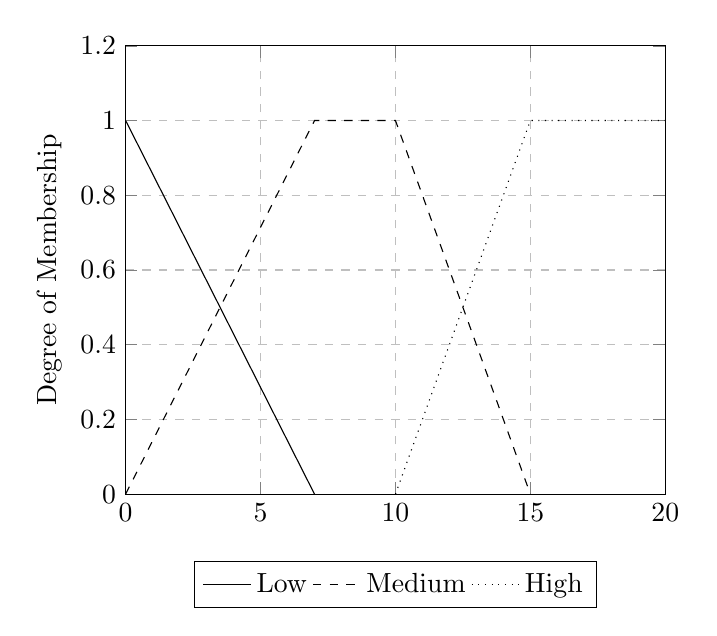
\begin{tikzpicture}
        \begin{axis}[
            ylabel={Degree of Membership},
            ymin=0, ymax=1.2,
            xmin=0, xmax=20,
            legend style={at={(0.5,-0.15)},anchor=north,legend columns=-1},
            ymajorgrids=true,
            xmajorgrids=true,
            grid style=dashed
        ]
        
        \addplot[solid, black] coordinates {(0,1) (0,1) (7,0)};
        \addlegendentry{Low}
        \addplot[dashed, black] coordinates {(0,0) (7,1) (10,1) (15,0)};
        \addlegendentry{Medium}
        \addplot[dotted, black] coordinates {(10,0) (15,1) (20,1)};
        \addlegendentry{High}
        
        \end{axis}
    \end{tikzpicture}
    \caption{Membership Function for Phish Hints}
\end{figure}

\textbf{Domain Age}
\begin{itemize}
    \item \textbf{Description:} Age of the website in months.  
    \item \textbf{Type:} Integer  
    \item \textbf{Reference:} Feature 83 in the paper  
\end{itemize}

\begin{figure}[H]
    \centering
    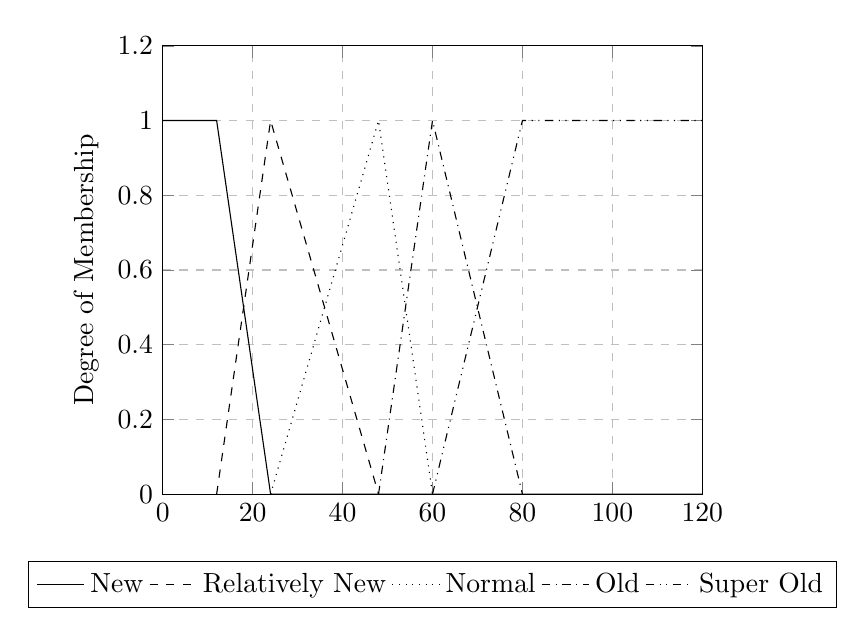
\begin{tikzpicture}
        \begin{axis}[
            ylabel={Degree of Membership},
            ymin=0, ymax=1.2,
            xmin=0, xmax=120,
            legend style={at={(0.5,-0.15)},anchor=north,legend columns=-1},
            ymajorgrids=true,
            xmajorgrids=true,
            grid style=dashed
        ]
        
        \addplot[solid, black] coordinates {(0,1) (12,1) (24,0) (120,0)};
        \addlegendentry{New}
        \addplot[dashed, black] coordinates {(12,0) (24,1) (48,0)};
        \addlegendentry{Relatively New}
        \addplot[dotted, black] coordinates {(24,0) (48,1) (60,0)};
        \addlegendentry{Normal}
        \addplot[dash dot, black] coordinates {(48,0) (60,1) (80,0)};
        \addlegendentry{Old}
        \addplot[dash dot dot, black] coordinates {(60,0) (80,1) (120,1)};
        \addlegendentry{Super Old}
        
        \end{axis}
    \end{tikzpicture}
    \caption{Membership Function for Domain Age (in months)}
\end{figure}

\subsubsection{Content Features}
\textbf{Ratio of External Hyperlinks}
\begin{itemize}
    \item \textbf{Description:} The number of external hyperlinks on a webpage divided by the total number of hyperlinks.  
    \item \textbf{Type:} Float  
    \item \textbf{Reference:} Feature 59 in the paper  
\end{itemize}

\begin{figure}[H]
    \centering
    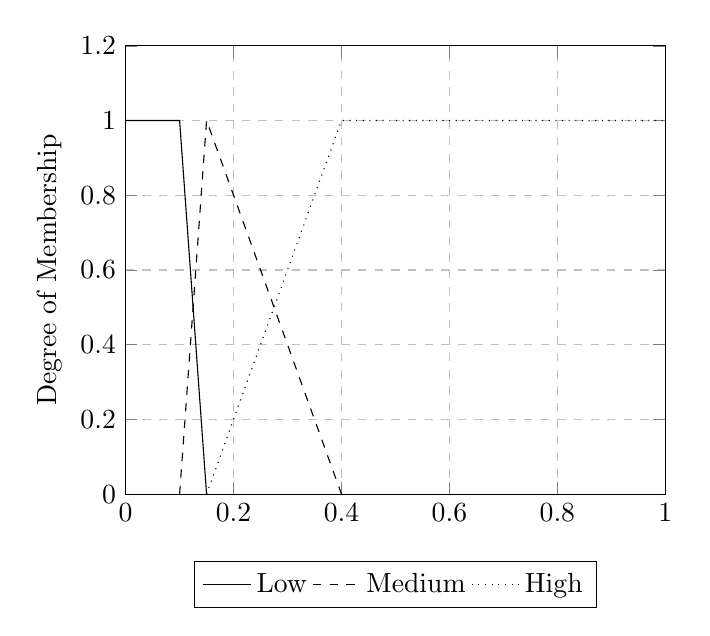
\begin{tikzpicture}
        \begin{axis}[
            ylabel={Degree of Membership},
            ymin=0, ymax=1.2,
            xmin=0, xmax=1,
            legend style={at={(0.5,-0.15)},anchor=north,legend columns=-1},
            ymajorgrids=true,
            xmajorgrids=true,
            grid style=dashed
        ]
        
        \addplot[solid, black] coordinates {(0,1) (0.1,1) (0.15,0)};
        \addlegendentry{Low}
        \addplot[dashed, black] coordinates {(0.1,0) (0.15,1) (0.4,0)};
        \addlegendentry{Medium}
        \addplot[dotted, black] coordinates {(0.15,0) (0.4,1) (1,1)};
        \addlegendentry{High}
        
        \end{axis}
    \end{tikzpicture}
    \caption{Membership Function for Ratio of External Hyperlinks}
\end{figure}

\subsubsection{External Features}
\textbf{Google Index}
\begin{itemize}
    \item \textbf{Description:} Indicates whether a webpage is indexed by Google.  
    \item \textbf{Type:} Boolean  
    \item \textbf{Reference:} Feature 86 in the paper  
\end{itemize}

\begin{figure}[H]
    \centering
    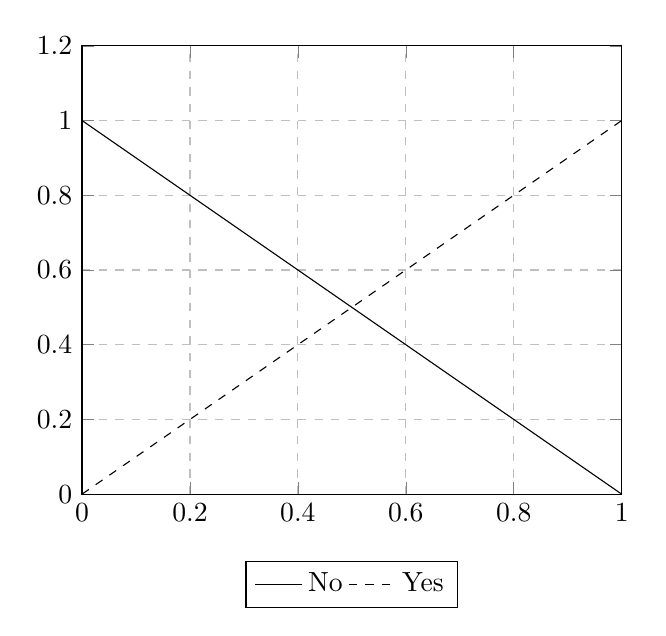
\begin{tikzpicture}
        \begin{axis}[
            ymin=0, ymax=1.2,
            xmin=0, xmax=1,
            legend style={at={(0.5,-0.15)},anchor=north,legend columns=-1},
            ymajorgrids=true,
            xmajorgrids=true,
            grid style=dashed
        ]
        
        \addplot[solid, black] coordinates {(0,1) (1,0)};
        \addlegendentry{No}
        \addplot[dashed, black] coordinates {(0,0) (1,1)};
        \addlegendentry{Yes}
        
        \end{axis}
    \end{tikzpicture}
    \caption{Membership Function for Google Index}
\end{figure}

\textbf{GTR}
\begin{itemize}
    \item \textbf{Description:} Google Toolbar Rank, a value from 0 to 10 that reflects the importance of the webpage.  
    \item \textbf{Type:} Integer  
    \item \textbf{Reference:} Feature 87 in the paper  
\end{itemize}

\begin{figure}[H]
    \centering
    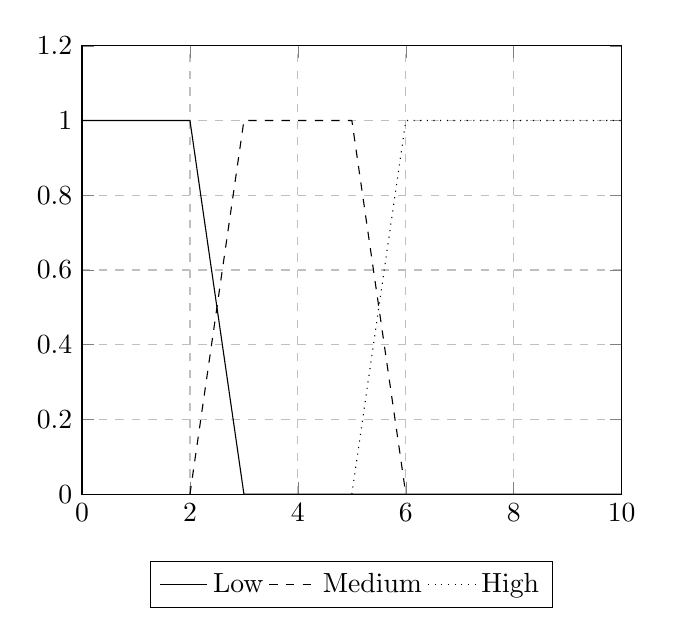
\begin{tikzpicture}
        \begin{axis}[
            ymin=0, ymax=1.2,
            xmin=0, xmax=10,
            legend style={at={(0.5,-0.15)},anchor=north,legend columns=-1},
            ymajorgrids=true,
            xmajorgrids=true,
            grid style=dashed
        ]
        
        \addplot[solid, black] coordinates {(0,1) (2,1) (3,0) (10,0)};
        \addlegendentry{Low}
        \addplot[dashed, black] coordinates {(2,0) (3,1) (5,1) (6,0)};
        \addlegendentry{Medium}
        \addplot[dotted, black] coordinates {(5,0) (6,1) (10,1)};
        \addlegendentry{High}
        
        \end{axis}
    \end{tikzpicture}
    \caption{Membership Function for Google Toolbar Rank (GTR)}
\end{figure}

\section{Output Variable}
The output variable represents the phishing risk. It is classified into four fuzzy sets, as illustrated in Figure \ref{output_variable}.

\begin{figure}[H]
    \centering
    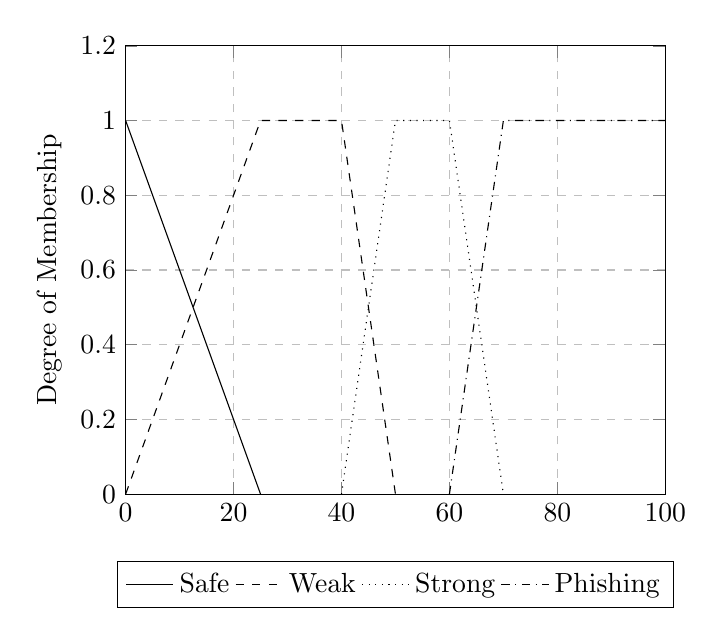
\begin{tikzpicture}
        \begin{axis}[
            ylabel={Degree of Membership},
            ymin=0, ymax=1.2,
            xmin=0, xmax=100,
            legend style={at={(0.5,-0.15)},anchor=north,legend columns=-1},
            ymajorgrids=true,
            xmajorgrids=true,
            grid style=dashed
        ]
        
        \addplot[solid, black] coordinates {(0,1) (0,1) (25,0)};
        \addlegendentry{Safe}
        \addplot[dashed, black] coordinates {(0,0) (25,1) (40,1) (50,0)};
        \addlegendentry{Weak}
        \addplot[dotted, black] coordinates {(40,0) (50,1) (60,1) (70,0)};
        \addlegendentry{Strong}
        \addplot[dash dot, black] coordinates {(60,0) (70,1) (100,1)};
        \addlegendentry{Phishing}
        
        \end{axis}
    \end{tikzpicture}
    \caption{Membership Function for Phishing Risk (Output Variable)}
    \label{output_variable}
\end{figure}

\section{Implementation}
In our implementation, we utilized the MATLAB Fuzzy Logic Toolbox to develop the fuzzy expert system. The system was designed using the Mamdani fuzzy inference method, which is well-suited for decision-making processes that require a human-like reasoning approach. In this system, we employed the minimum (min) operation as the t-norm for the intersection of fuzzy sets, and the maximum (max) operation as the t-conorm for the union of fuzzy sets. For the defuzzification process, we selected the Center of Area (CoA) method, which calculates the centroid of the aggregated fuzzy set to produce a crisp output. This approach ensures that the output is a balanced representation of the input conditions, providing a reliable decision-making framework for detecting phishing websites.

To validate the fuzzy expert system, we employed the MATLAB 3D plot. As this plot only allows the representation of 2 inputs and the output at a time, we viewed the 10 possible combinations, all of which were consistent. At the same time, every possible combination was covered, as no combination was left without a rule being activated.

\section{Rules}

To design the rules involving Google Index, we consulted~\cite{mainpaper}, which states that pages not indexed by Google are more likely to be phishing websites. Consequently, we devised the rules listed in Table \ref{google_index_rules}.

\begin{table}[H]
    \centering
    \begin{tabular}{|l|l|l|}
        \hline
        \textbf{Google Index} & \textbf{Phishing Risk} & \textbf{Weight} \\ \hline
        NO                    & PHISHY                 & 1               \\ \hline
        YES                   & WEAK                   & 1               \\ \hline
    \end{tabular}
    \caption{Rules for Google Index}
    \label{google_index_rules}
\end{table}

For the GTR, we consulted~\cite{GTR}, which states:

\begin{quote}
    \textit{GTR value is considered as a heuristic because the PageRank value for legitimate sites will be high, whereas for phishing pages, its value will be lower.}
\end{quote}

Regarding Phish Hints, \cite{mainpaper} explains that a higher number of Phish Hints in a URL indicates a greater likelihood of the website being a phishing site. Accordingly, we defined the rules in Table \ref{page_rank_phish_hints_rules}.

\begin{table}[h]
    \centering
    \begin{tabular}{|l|l|l|l|l|}
    \hline
    \textbf{GTR} & \textbf{Phish Hints} & \textbf{Operator} & \textbf{Phishing Risk} & \textbf{Weight} \\ \hline
    HIGH               &                     &                   & SAFE                   & 1               \\ \hline
    MEDIUM             & LOW                 & AND               & WEAK                   & 0.5             \\ \hline
    MEDIUM             & MEDIUM              & AND               & STRONG                 & 1               \\ \hline
    MEDIUM             & HIGH                & AND               & PHISHY                 & 1               \\ \hline
    LOW                & LOW                 & AND               & STRONG                 & 0.5             \\ \hline
    LOW                & MEDIUM              & AND               & STRONG                 & 1               \\ \hline
    LOW                & HIGH                & AND               & PHISHY                 & 1               \\ \hline
    \end{tabular}
    \caption{Rules for GTR and Phish Hints}
    \label{page_rank_phish_hints_rules}
\end{table}

To evaluate the effect of the domain age feature, we consulted~\cite{domainage}, which states:

\begin{quote}
\textit{The top feature in the list is domain age, which confirms our assumptions that long-running services are statistically more credible.}
\end{quote}

Thus, we consider older domains less likely to be phishing websites. Similarly, to assess the effect of the ratio of external hyperlinks, we consulted~\cite{externalhyperlinks}, which notes:

\begin{quote}
\textit{Phishing websites often include numerous external hyperlinks pointing to target websites because cybercriminals frequently replicate the HTML code from legitimate websites to construct their phishing sites.}
\end{quote}

All this information led to the creation of the rules in Table \ref{domainage_hyperlinks_rules}.

\begin{table}[H]
    \centering
    \begin{tabular}{|l|l|l|l|l|}
    \hline
    \textbf{Domain Age}     & \textbf{Ratio of Hyperlinks} & \textbf{Operator} & \textbf{Phishing Risk} & \textbf{Weight} \\ \hline
    SUPER OLD      &                     &                   & SAFE                   & 1               \\ \hline
    OLD            & LOW                 & OR                & SAFE                   & 0.5             \\ \hline
    NORMAL         & LOW                 & AND               & WEAK                   & 0.5             \\ \hline
    NORMAL         & MEDIUM              & AND               & STRONG                 & 0.5             \\ \hline
    NORMAL         & HIGH                & AND               & STRONG                 & 0.5             \\ \hline
    RELATIVELY NEW & LOW                 & AND               & WEAK                   & 1               \\ \hline
    RELATIVELY NEW & MEDIUM              & AND               & STRONG                 & 1               \\ \hline
    RELATIVELY NEW & HIGH                & AND               & PHISHY                 & 0.5             \\ \hline
    NEW            & LOW                 & AND               & STRONG                 & 0.5             \\ \hline
    NEW            & MEDIUM              & AND               & STRONG                 & 1               \\ \hline
    NEW            & HIGH                & AND               & PHISHY                 & 1               \\ \hline
    \end{tabular}
    \caption{Rules for Domain Age and Ratio of External Hyperlinks}
    \label{domainage_hyperlinks_rules}
\end{table}

\section{Implementation}

In our implementation, we utilized the MATLAB Fuzzy Logic Toolbox to develop the fuzzy expert system. The system was designed using the Mamdani fuzzy inference method, which is well-suited for decision-making processes requiring human-like reasoning. In this system, we employed the minimum (min) operation as the t-norm for the intersection of fuzzy sets, and the maximum (max) operation as the t-conorm for the union of fuzzy sets. For the defuzzification process, we selected the Center of Area (CoA) method, which calculates the centroid of the aggregated fuzzy set to produce a crisp output. This approach ensures that the output is a balanced representation of the input conditions, providing a reliable decision-making framework for detecting phishing websites.

To validate the fuzzy expert system, we employed MATLAB 3D plots. As these plots only allow the representation of two inputs and the output at a time, we analyzed all ten possible combinations. The results were consistent, with no combinations left without an activated rule.


\section{Testing}

This section presents the testing of the fuzzy system. Four test cases, representing different scenarios, are evaluated. Some cases are designed to activate multiple rules. The results of each test case are reported with screenshots and explanations to justify the obtained outputs, including the activations of the rules. In the screenshots, we only provide the rules that are activated in each case.

\subsection{Test Cases}

The dataset used by ~\cite{mainpaper} includes legitimate and phishing websites. Finding phishing websites that are still active was challenging, as they are often unavailable for extended periods. For the domain age, the data provided in the dataset (accurate at the time of creation) was used.

\subsubsection{Case 1: Phishing Website}

\begin{itemize}
    \item \textbf{URL:} \url{https://dichvuvnpt.com/home/components/com_user/bbtonline.html}
    \item \textbf{Personal Opinion:} The site appears suspicious at first glance, as the formatting seems a bit off. The URL is also suspicious, but it is not immediately obvious that it is phishing.
    \item \textbf{Attributes:}
    \begin{itemize}
        \item Domain Age: $3767$ hours $= 7.1$ months
        \item Phish Hints: $0$
        \item Ratio of External Hyperlinks: $1.0$
        \item Google Index: $1$
        \item GTR: $0$
    \end{itemize}
    \begin{figure}[h!]
        \centering
        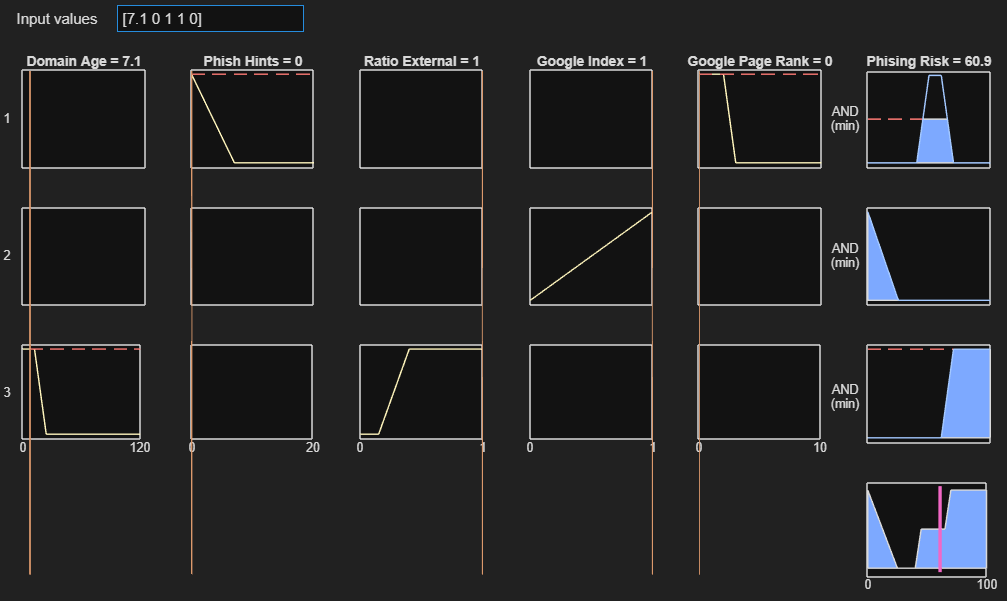
\includegraphics[width=\textwidth]{test-1.png}
        \caption{Test Case 1: Phishing Website}
    \end{figure}
    \item \textbf{Rules Activated:} 
    \begin{itemize}
        \item \textbf{Rule 5:} If Phish Hints is Low and Google GTR is Low, then Phishing Risk is Strong
        \item \textbf{Rule 9:} If Google Index is Yes, then Phishing Risk is Safe
        \item \textbf{Rule 20:} If Domain Age is New and Ratio of External Hyperlinks is High, then Phishing Risk is Phishing
    \end{itemize}
    \item \textbf{Output:} $60.9$
    \item Classification for 60.9: \textbf{Strong} (with membership 1)
\end{itemize}

We see that the Google Index is not a clear indicator of phishing, as the site is indexed but still classified as phishing. The high ratio of external hyperlinks and relatively new domain age are the main factors leading to this classification.

\subsubsection{Case 2: Phishing Website}

\begin{itemize}
    \item \textbf{URL:} \url{https://www.courgeon-immobilier.fr/} (line 6593)
    \item \textbf{Personal Opinion:} The site initially appears professional and trustworthy. However, closer inspection reveals phishing behavior (e.g., fake social media links).
    \item \textbf{Attributes:}
    \begin{itemize}
        \item Domain Age: $2300$ hours $= 3.15$ months
        \item Phish Hints: $2$
        \item Ratio of External Hyperlinks: $0.4545$
        \item Google Index: $1$
        \item GTR: $2$
    \end{itemize}
    \begin{figure}[h!]
        \centering
        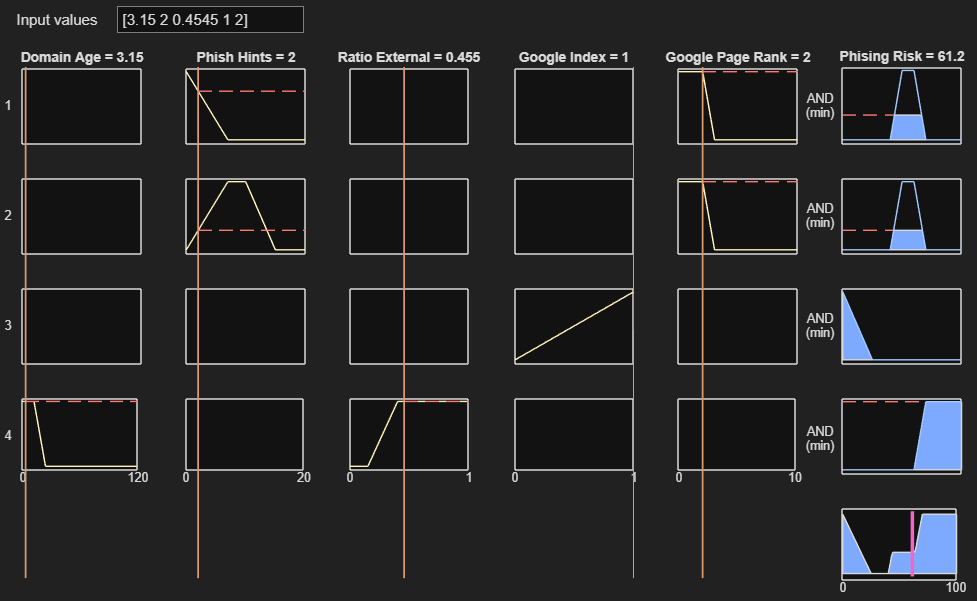
\includegraphics[width=\textwidth]{test-2.png}
        \caption{Test Case 2: Phishing Website}
    \end{figure}
    \item \textbf{Rules Activated:} 
    \begin{itemize}
        \item \textbf{Rule 5:} If Phish Hints is Low and Google GTR is Low, then Phishing Risk is Strong
        \item \textbf{Rule 6:} If Phish Hints is Medium and Google GTR is Low, then Phishing Risk is Strong
        \item \textbf{Rule 9:} If Google Index is Yes, then Phishing Risk is Safe
        \item \textbf{Rule 20:} If Domain Age is New and Ratio of External Hyperlinks is High, then Phishing Risk is Phishing
    \end{itemize}
    \item \textbf{Output:} $61.2$
    \item Classification for 61.2: \textbf{Phishing} (with membership 1)
\end{itemize}

The site is classified as phishing due to its relatively new domain age, high ratio of external hyperlinks, and the presence of phishing hints. The Google GTR is low, but the Google Index is active again, which does not seem to be a strong indicator of phishing.

\subsubsection{Case 3: Legitimate Website}

\begin{itemize}
    \item \textbf{URL:} \url{https://www.physiologyweb.com/lecture_notes/membrane_transport/secondary_active_transport.html} (line 6598)
    \item \textbf{Personal Opinion:} The site is for educational purposes, and it would be unexpected for it to be phishing. 
    \item \textbf{Attributes:}
    \begin{itemize}
        \item Domain Age: $3596$ hours $= 4.92$ months
        \item Phish Hints: $0$
        \item Ratio of External Hyperlinks: $0.1428$
        \item Google Index: $0$
        \item GTR: $4$
    \end{itemize}
    \begin{figure}[h!]
        \centering
        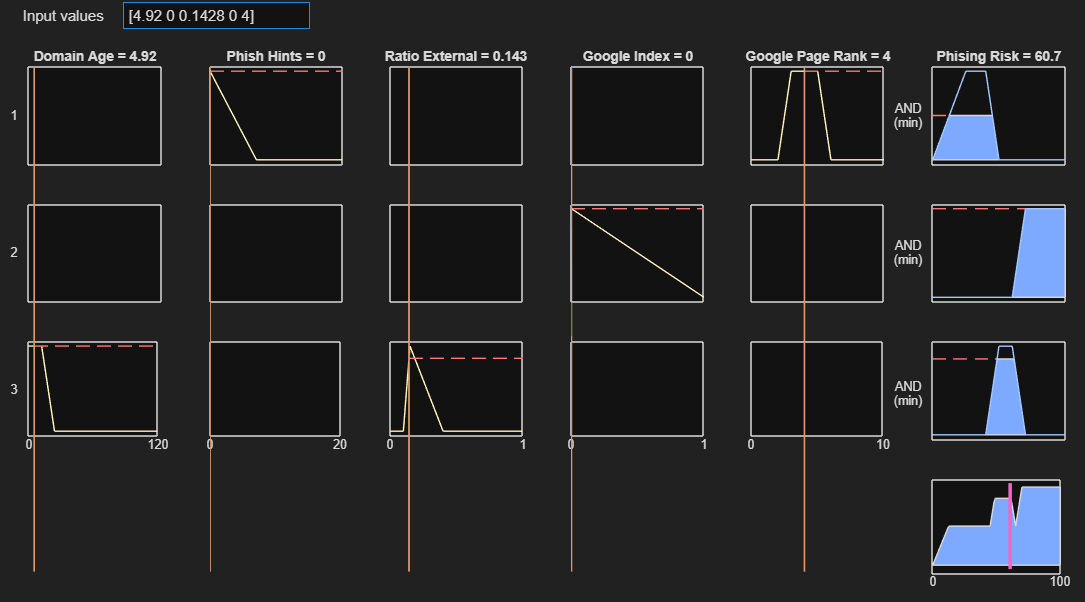
\includegraphics[width=\textwidth]{test-3.png}
        \caption{Test Case 3: Legitimate Website (False Positive)}
    \end{figure}
    \item \textbf{Rules Activated:} 
    \begin{itemize}
        \item \textbf{Rule 2:} If Phish Hints is Low and Google GTR is Medium, then Phishing Risk is Weak
        \item \textbf{Rule 8:} If Google Index is No, then Phishing Risk is Phishing
        \item \textbf{Rule 19:} If Domain Age is Normal and Ratio of External Hyperlinks is Low, then Phishing Risk is Weak
    \end{itemize}
    \item \textbf{Output:} $60.7$
    \item Classification for 60.7: \textbf{Phishing} (with membership 0.9825), but Strong is also active with membership 1
\end{itemize}

Despite being a legitimate site, the system classifies it as likely phishing due to its relatively recent creation and lack of Google indexing. This is a false positive, as the site is a legitimate educational resource. 

\subsubsection{Case 4: Legitimate Website}

\begin{itemize}
    \item \textbf{URL:} \url{https://en.wikipedia.org/wiki/Aurelio_Voltaire} (line 6638)
    \item \textbf{Personal Opinion:} As Wikipedia is a well-known and trustworthy site, it is expected to be classified as legitimate.
    \item \textbf{Attributes:}
    \begin{itemize}
        \item Domain Age: $7132$ hours $= 9.8$ months
        \item Phish Hints: $0$
        \item Ratio of External Hyperlinks: $0.1305$
        \item Google Index: $1$
        \item GTR: $7$
    \end{itemize}
    \begin{figure}[h!]
        \centering
        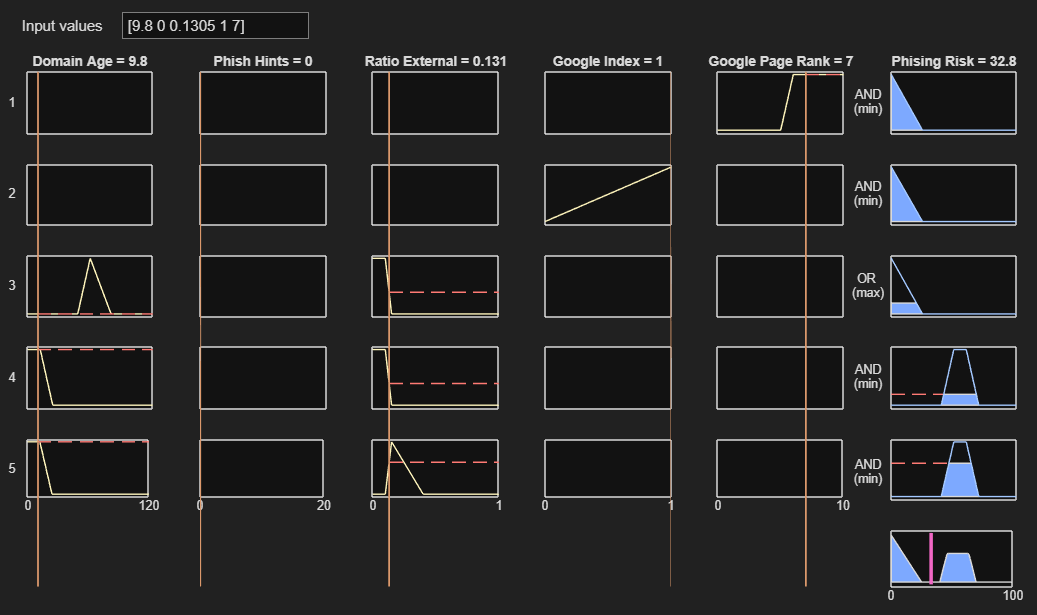
\includegraphics[width=\textwidth]{test-4.png}
        \caption{Test Case 4: Legitimate Website}
    \end{figure}
    \item \textbf{Rules Activated:} 
    \begin{itemize}
        \item \textbf{Rule 1:} If Google GTR is High, then Phishing Risk is Safe
        \item \textbf{Rule 9:} If Google Index is Yes, then Phishing Risk is Safe
        \item \textbf{Rule 11:} If Domain Age is Old or Ratio of External Hyperlinks is Low, then Phishing Risk is Safe
        \item \textbf{Rule 18:} If Domain Age is New and Ratio of External Hyperlinks is Low, then Phishing Risk is Strong
        \item \textbf{Rule 19:} If Domain Age is Normal and Ratio of External Hyperlinks is Low, then Phishing Risk is Weak
    \end{itemize}
    \item \textbf{Output:} $32.8$
    \item Classification for 32.8: \textbf{Weak} (with membership 0.52)
\end{itemize}

The high Google GTR is a strong indicator of legitimacy. The site also has a low ratio of external hyperlinks, which is another indicator of trustworthiness. The site is classified as weak, which is expected for a well-known site like Wikipedia.

\section{Complex Fuzzy Expert System}

This fuzzy expert system is structured into two hierarchical layers. The first layer consists of three independent Mamdani fuzzy systems, each focusing on a specific dimension of a website: \textbf{URL-based features}, \textbf{Content-based features}, and \textbf{External-based features}. The outputs from these three systems are then combined in a second-layer Mamdani fuzzy system to compute the overall phishing risk score.

\subsection{Layer 1: Feature-Based Risk Assessments}

The first layer is composed of three Mamdani fuzzy inference systems, each focusing on a specific feature category. These systems process their respective input features to generate risk levels as outputs:

\begin{itemize}
    \item URL Risk Mamdani System: 
    
    This system evaluates whether characteristics of the URL indicate phishing behavior, such as excessively long URLs or unusual characters.

    Examples of outputs include:
    \begin{itemize}
        \item URL Length (f1-f2)
        \item Special Characters in the URL(f4-f20)
    \end{itemize}

    \item Content Risk Mamdani System:
    
    This system identifies suspicious behaviors in the webpage content, such as malicious forms or hidden elements designed to deceive users.

    Examples of outputs include:
    \begin{itemize}
        \item Number of Hyperlinks (f57)
        \item Login Form Actions (f66)
        \item Presence of Invisible Iframes (f73)
    \end{itemize}

    \item External Risk Mamdani System:
    
    This system assesses external attributes that provide context for the website's legitimacy, such as its age or popularity.

    Examples of outputs include:
    \begin{itemize}
        \item Domain Age (f83)
        \item Google Index Presence (f86)
        \item Web Traffic Volume (f84)
    \end{itemize}

\end{itemize}

\subsection{Layer 2: Overall Phishing Risk Assessment}

The second layer takes the outputs from the first layer (URL Risk, Content Risk, External Risk) and combines them into an overall phishing risk score using another Mamdani fuzzy inference system. Each of these risks carries a specific weight, reflecting its relative importance in detecting phishing. The weights are designed to balance sensitivity (detecting as many phishing websites as possible) and precision (minimizing false positives).

\subsection{Weight Distribution}

The importance of each risk category (URL, Content, External) varies based on its correlation with phishing behavior. By assigning appropriate weights, the system can prioritize the most reliable and significant indicators:

\begin{itemize}
    \item URL Risk (40\%-50\%):
    
    This category carries the highest weight because a suspicious URL alone can often be enough to classify a website as high-risk. However, legitimate websites may also have long or unusual URLs, so this weight must be carefully balanced.

    \item Content Risk (30\%-40\%):
    
    This category carries slightly less weight than URL risk because, while content indicators are highly relevant, legitimate websites can occasionally exhibit similar patterns (e.g., a minimalist design with few links). Nonetheless, content risk remains a strong contributing factor.

    \item External Risk (20\%-30\%):
    
    External risks carry the lowest weight because they are indirect indicators. While they add valuable context, they are less conclusive compared to URL or content risks.

\end{itemize}


\begin{figure}[h!]
    \centering
    \begin{tikzpicture}[scale=.8,auto=left, node style/.style={draw, ellipse, minimum width=3.2cm, minimum height=1cm}]
        % Nodes
        \node[node style, fill=cyan!30] (n6) at (-2,12) {URL-based features};
        \node[node style, fill=cyan!30] (n4) at (-2,7)  {Content features};
        \node[node style, fill=cyan!30] (n5) at (-2,2)  {External features};
        \node[node style, fill=orange!30] (n1) at (7,10) {URL Risk};
        \node[node style, fill=orange!30] (n2) at (7,7)  {Content Risk};
        \node[node style, fill=orange!30] (n3) at (7,4)  {External Risk};
        \node[node style, fill=red!30] (n7) at (17,7) {Phishing Risk};

        % rules blocks
        \node[draw, rectangle, minimum width=3cm, minimum height=1cm, fill=yellow!30] (r1) at (2.5,11) {Rule Block 1};
        \node[draw, rectangle, minimum width=3cm, minimum height=1cm, fill=yellow!30] (r2) at (2.5,7) {Rule Block 2};
        \node[draw, rectangle, minimum width=3cm, minimum height=1cm, fill=yellow!30] (r3) at (2.5,3) {Rule Block 3};
        \node[draw, rectangle, minimum width=3cm, minimum height=1cm, fill=yellow!30] (r4) at (12,7) {Final Rule Block};

        % Connections
        \draw (n6) -- (r1);
        \draw (r1) -- (n1);
        \draw (n4) -- (r2);
        \draw (r2) -- (n2);
        \draw (n5) -- (r3);
        \draw (r3) -- (n3);
        \draw (n1) -- (r4);
        \draw (n2) -- (r4);
        \draw (n3) -- (r4);
        \draw (r4) -- (n7);

        \node[draw, rectangle, minimum width=1cm, minimum height=0.5cm, fill=cyan!30] at (11,5) {};
        \node at (14,5) {Input Features};

        \node[draw, rectangle, minimum width=1cm, minimum height=0.5cm, fill=yellow!30] at (11,4) {};
        \node at (14,4) {Rule Blocks};

        \node[draw, rectangle, minimum width=1cm, minimum height=0.5cm, fill=orange!30] at (11,3) {};
        \node at (15,3) {Intermediate Outputs (Risks)};

        \node[draw, rectangle, minimum width=1cm, minimum height=0.5cm, fill=red!30] at (11,2) {};
        \node at (15, 2) {Final Output (Phishing Risk)};


    \end{tikzpicture}
    \caption{Hierarchical Fuzzy Expert System for Phishing Detection with Rule Blocks}
    \label{fig:phishing_system_with_rules}
\end{figure}
% Bibliography
\newpage
\printbibliography


\end{document}